%   MSc Business Analytics Dissertation
%   Format based on skeleton template provided as part of module MIS40750
%
%   Title:     Optimising the design of buffer preparation in bioprocessing
%              facilities
%   Author:    Sean Tully
%
%   Appendix 3: real-world example 2
%
%   Change Control:
%   When     Who   Ver  What
%   -------  ----  ---  --------------------------------------------------------

\chapter{Real-world data set 2}\label{C.real2}

\begin{table}[h]
    \centering Table A4: Buffer data for real-world data set 2\\
    \label{tbl.buffer2}
    \begin{tabular}{l | c | c | c}
        names & required volumes & use start times & use durations\\
        & $U_{n}$ (l) & $t_{\mathit{USE},n}^{*}$ (h) 
        & $\Delta t_{\mathit{USE},n}$
        (h)\\ \hline
        \text{Buffer \#1} & \SI{72.0}{} & \SI{93.75}{} & \SI{4.86}{}\\
        \text{Buffer \#2} & \SI{208.0}{} & \SI{86.72}{} & \SI{9.19}{}\\
        \text{Buffer \#3} & \SI{242.0}{} & \SI{36.57}{} & \SI{3.51}{}\\
        \text{Buffer \#4} & \SI{453.0}{} & \SI{73.51}{} & \SI{5.59}{}\\
        \text{Buffer \#5} & \SI{478.0}{} & \SI{83.76}{} & \SI{4.95}{}\\
        \text{Buffer \#6} & \SI{567.0}{} & \SI{68.78}{} & \SI{2.29}{}\\
        \text{Buffer \#7} & \SI{618.0}{} & \SI{28.01}{} & \SI{1.89}{}\\
        \text{Buffer \#8} & \SI{810.0}{} & \SI{110.57}{} & \SI{2.79}{}\\
        \text{Buffer \#9} & \SI{845.0}{} & \SI{110.21}{} & \SI{31.68}{}\\
        \text{Buffer \#10} & \SI{1107.0}{} & \SI{112.46}{} & \SI{37.65}{}\\
        \text{Buffer \#11} & \SI{1203.0}{} & \SI{98.62}{} & \SI{1.62}{}\\
        \text{Buffer \#12} & \SI{1639.0}{} & \SI{66.43}{} & \SI{22.29}{}\\
        \text{Buffer \#13} & \SI{1772.0}{} & \SI{110.93}{} & \SI{39.19}{}\\
        \text{Buffer \#14} & \SI{2128.0}{} & \SI{26.06}{} & \SI{4.05}{}\\
        \text{Buffer \#15} & \SI{2171.0}{} & \SI{66.97}{} & \SI{21.75}{}\\
        \text{Buffer \#16} & \SI{3873.0}{} & \SI{36.66}{} & \SI{48.39}{}\\
        \text{Buffer \#17} & \SI{4503.0}{} & \SI{44.42}{} & \SI{35.76}{}\\
        \text{Buffer \#18} & \SI{4987.0}{} & \SI{94.05}{} & \SI{12.97}{}\\
        \text{Buffer \#19} & \SI{5826.0}{} & \SI{103.81}{} & \SI{47.39}{}\\
        \text{Buffer \#20} & \SI{6225.0}{} & \SI{111.65}{} & \SI{32.39}{}\\
        \text{Buffer \#21} & \SI{10682.0}{} & \SI{42.16}{} & \SI{40.72}{}\\
        \text{Buffer \#22} & \SI{14253.0}{} & \SI{99.16}{} & \SI{13.63}{}\\
    \end{tabular}
\end{table}

\begin{table}[h]
    \centering Table A5: Vessel data for real-world data set 2\\
    \label{tbl.vessel2}
    \begin{tabular}{l | r | r}
        names & volumes & costs\\
        & $V_{m}$ (l) & $c_{m}$ (--)\\\hline
        \SI{100}{\litre} & \SI{100.0}{} & \SI{15.85}{}\\
        \SI{200}{\litre} & \SI{200.0}{} & \SI{24.02}{}\\
        \SI{500}{\litre} & \SI{500.0}{} & \SI{41.63}{}\\
        \SI{1000}{\litre} & \SI{1000.0}{} & \SI{63.10}{}\\
        \SI{2500}{\litre} & \SI{2500.0}{} & \SI{109.34}{}\\
        \SI{5000}{\litre} & \SI{5000.0}{} & \SI{165.72}{}\\
        \SI{7500}{\litre} & \SI{7500.0}{} & \SI{211.37}{}\\
        \SI{10000}{\litre} & \SI{10000.0}{} & \SI{251.19}{}\\
        \SI{15000}{\litre} & \SI{15000.0}{} & \SI{320.37}{}\\
    \end{tabular}
\end{table}

\begin{table}[h!]
    \centering Table A6: Global parameters for real-world data set 2
    \label{tbl.parameters2}
    \begin{tabular}{l | l | r | c}
        symbol & short description & value & unit\\ \hline
        $T$ & process cycle time & 120.0 & h\\
        $\Delta t_{\mathit{PREP,PRE}}$ & prep pre duration & 10.3 & h\\
        $\Delta t_{\mathit{PREP,POST}}$ & prep post duration & 2.7 & h\\
        $\Delta t_{\mathit{TRANSFER}}$ & transfer duration & 2.1 & h\\
        $\Delta t_{\mathit{HOLD,PRE}}$ & hold pre duration & 7.0 & h\\
        $\Delta t_{\mathit{HOLD,POST}}$ & hold post duration & 2.2 & h\\
        $\Delta t_{\mathit{HOLD,MIN}}$ & minimum hold duration & 1.0 & h\\
        $\Delta t_{\mathit{HOLD,MAX}}$ & maximum hold duration & 60.0 & h\\
        $f_{\mathit{MINFILL}}$ & minimum fill ratio & 0.3 & --\\
        $f_{\mathit{UTIL}}$ & maximum utilisation ratio & 0.8 & --\\
    \end{tabular}
\end{table}

\begin{figure}[h]
    \centering
    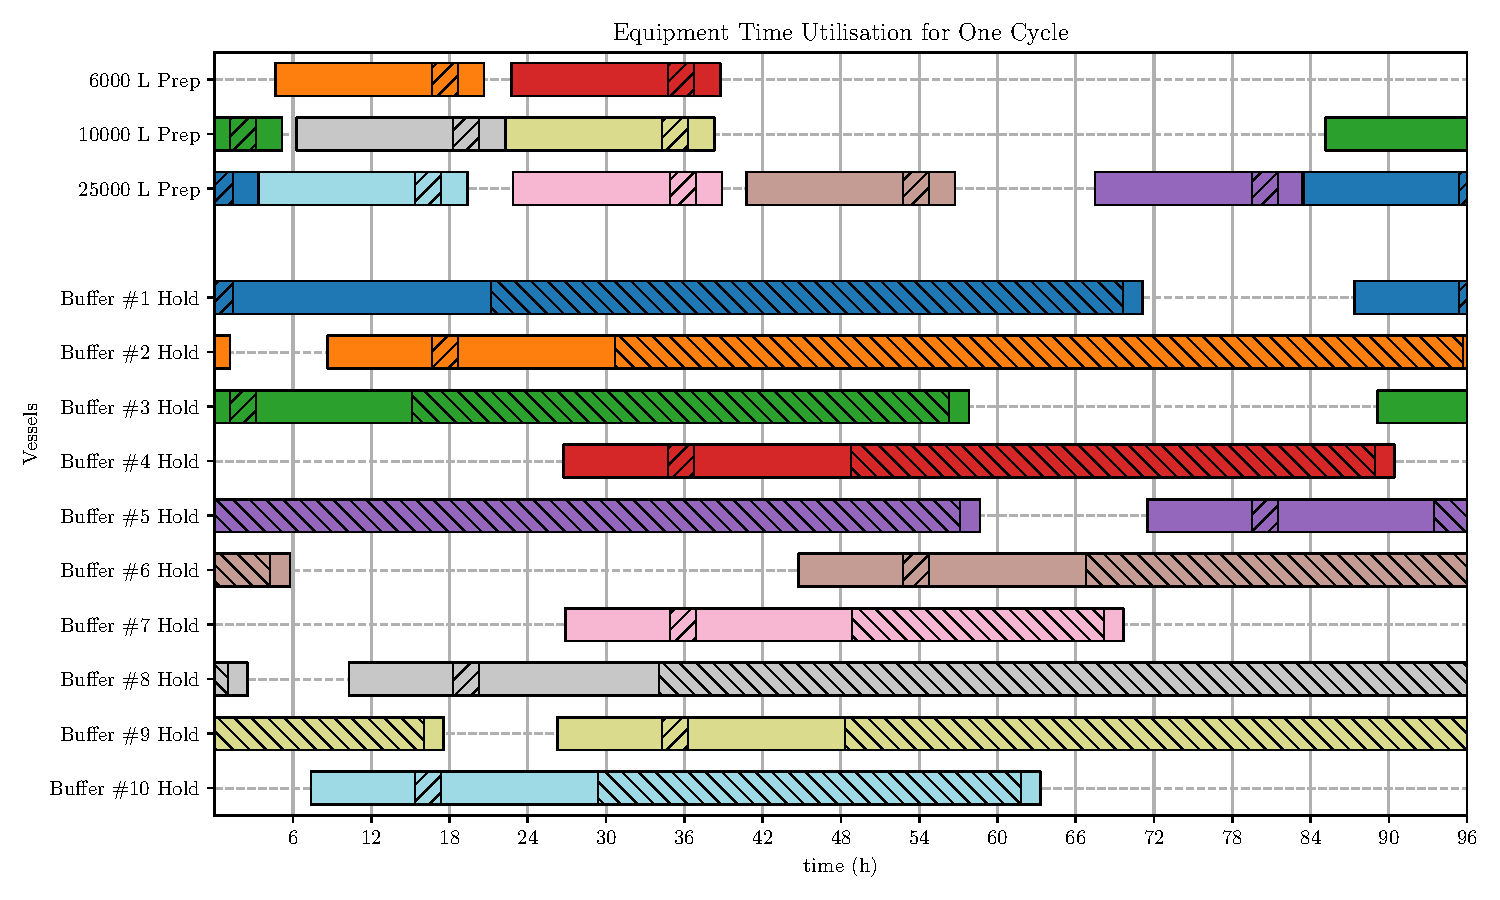
\includegraphics[width=\linewidth]{../examples/plant2/plot2.pdf}
    Figure A2: Real-world data set 2 -- complete model with minimised
        hold times
    \label{fig.secondary1}
\end{figure}
